% paper_hinge_appendix.tex — the hinge appendix for the eight-bot zoo (2026-10-13). Numbers from
% app/generated/egt/runs/body8_sprime[_hinge_side]_t100_a030_*; EGT_FINDINGS_SPRIME.md §8.4. Table: figures and tables/hinge_body_compare.tex.
\subsubsection{Hinge results}
\label{apx-subsubsection:Experiments-BaseBots-Hinge}
On the hinge side the counts are 24, 18 and 22, with 35 row actions $C$: the open question moves six cells, four of them to mutual cooperation (\texttt{DupocBot} stops exploiting the else-branch cooperators \texttt{DBot} and \texttt{EBot}) and two to mutual defection (\texttt{CupodBot}'s detector fires on \texttt{OBot}).

\paragraph{Robustness to the hinge.} Every number of \cref{section:Results-Base} takes the three hinge pairs at the floor side. We re-ran the same stages with them at the hinge side; \cref{tab:hinge-body} puts the two branches side by side. The qualitative answer does not move: there is still no pure ESS, the three Nash components are still present (joined by two mixed ones, both carried by \texttt{EBot}, which the hinge side turns into a reciprocator of \texttt{DupocBot}), the dominant replicator support is the same, and at strong selection \texttt{DupocBot} is still the only stochastically stable strategy, at every $M$. What moves is the margin. \texttt{DupocBot} no longer exploits \texttt{DBot} and \texttt{EBot}, so its row loses two units of the temptation payoff; \texttt{TitForTatBot}, which already cooperated with both, closes part of the gap and ties it at two of the nine points. The stationary share at $(100, 1)$ falls from 86\% to 71\%, the cooperative basin from 88\% to 81\%, a small all-defect basin \{\texttt{DefectBot}, \texttt{OBot}\} appears with 4.5\% of the starts, and the self-cooperating share of the long run drops from 0.92 to 0.84. One structural change is worth a sentence: on the hinge side \texttt{CupodBot}'s row of actions coincides with \texttt{DupocBot}'s (both cooperate with every reciprocator and defect on \texttt{DefectBot} and \texttt{OBot}), although their columns do not, since \texttt{DupocBot} exploits \texttt{CupodBot}; a behavior-reading signal cannot tell them apart there. The direction is the general one: on the hinge side the Löbian cooperator is \emph{more} cooperative and \emph{less} fit, because the cells it loses are the ones in which it exploited partners it could not read. The strong-selection claim of \cref{section:Results-Base} is therefore unconditional, and the share and the robustness count are the floor-side numbers of a bracket whose other end is 71\% and five of nine points.
% figures and tables/hinge_body_compare.tex — the eight-bot zoo (body8) at t = 1 under both branches of its three hinge dichotomies.
% Sources: app/generated/egt/runs/body8_sprime_t100_a030_ddbeab7343c4 (floor side) and body8_sprime_hinge_side_t100_a030_125c88740d9d (hinge side);
% EGT_FINDINGS_SPRIME.md §8.4. "self-cooperating share" = stationary mass of the types whose self-play cell is (C,C).
\begin{table}[t]
\centering
\begin{tabular}{lcc}
\toprule
\texttt{body}, $t = 1$ & floor side & hinge side \\
\midrule
Nash components (extreme equilibria) & 3 (21) & 5 (16) \\
\texttt{DupocBot} share at $(M,\beta) = (100, 1)$ & 85.9\% & 71.2\% \\
\texttt{DefectBot} share at $(100, 1)$ & 4.5\% & 8.3\% \\
$(M,\beta)$ points where \{\texttt{DupocBot}\} is the selected set & 8 / 9 & 5 / 9 \\
self-cooperating share of the long run at $(100, 1)$ & 0.92 & 0.84 \\
\bottomrule
\end{tabular}
\caption{The eight-bot zoo at full transparency under the two branches of its three hinge dichotomies. Floor side: the floor guards are not provable within budget (the engine's stipulation, the value of \cref{table:outcome-matrix-body}). Hinge side: they are. On the hinge side \texttt{TitForTatBot} ties \texttt{DupocBot} at $(50, 0.1)$ and $(100, 0.01)$, and no type is stochastically stable at the two weakest points.}
\label{tab:hinge-body}
\end{table}


% ---- added 2026-10-14: the partial-transparency hinge check (body8, both families, hinge side). Sources:
% app/generated/egt/runs/body8_sprime_hinge_side*_t*; analysis_hinge_side/{tidy,nash_structure}.csv; generator
% latex/scripts/gen_tau_body.py hinge_side. Inputs: tau_coop_body_hinge_side, tau_phase_body_hinge_side,
% fig_tau_{summary,families}_body_hinge_side. Everything below is [MINE].
\subsubsection{Hinge results under partial transparency}
\label{apx-subsubsection:Experiments-Transparency-Hinge}
We re-ran the two body sweeps of \cref{section:Results-Transparency} with the three hinge pairs at the hinge side. At full transparency the population cooperates at 0.84 instead of 0.92 (\cref{tab:hinge-body}), and below it the picture is less robust than on the floor side, for a reason that is visible in the matrix before any dynamics: on the hinge side \texttt{CupodBot}'s and \texttt{DupocBot}'s own-action rows coincide, so the behavioral family cannot tell them apart and spreads \texttt{DupocBot}'s mass over the two from the first step below $t = 1$. Under that family (\cref{table:tau-phase-body-hinge-side}, \cref{fig:tau-summary-body-hinge-side}) the stochastically stable set is \{\texttt{Cup}, \texttt{Dup}\} on all of $t \in [0.2, 0.8]$ for $\alpha \le 0.45$, with the population cooperating at 0.84 to 0.91 down to $t = 0.2$ as on the floor side; but at $\alpha = 0.62$ cooperation falls to 0.39 already at $t = 0.8$ (the static ceiling drops to 0.61 there) and to 0.04 at $t = 0.4$, and at $\alpha = 0.8$ it is not even monotone, 0.39 at $t = 0.8$ and 0.94 at $t = 0.6$ (a \texttt{TitForTatBot} monoculture) before collapsing at $t = 0.4$. The syntactic family does not confuse the two (their sources differ by one leaf) and gives the cleaner picture: cooperation survives down to $t = 0.6$ at $\alpha = 0.3$, $0.4$ at $\alpha = 0.45$, $0.2$ at $\alpha = 0.62$ and $0.6$ at $\alpha = 0.8$, with the static and the dynamic collapse again coinciding at every $\alpha$. The two families disagree on the selected set at 16 of the 30 grid points, against 5 on the floor side.

So the robustness bracket is wider under transparency than at $t = 1$. What survives the hinge: cooperation is still what selection keeps at full transparency, still needs only a fraction of the information for a trusting population (20\% under either channel), and still collapses at the same transparency under the static and the dynamic criterion. What does not: the threshold for a cautious population, which is 40 to 60\% on the floor side under either channel and becomes channel-dependent on the hinge side, 20 to 60\% under source blur and as high as full transparency under behavior blur once $\alpha \ge 0.62$. The reason is the row twin the hinge creates, not the dynamics, and a roster that separates \texttt{CupodBot} from \texttt{DupocBot} on the hinge side (the trolls rung does) would remove it.
% figures and tables/tau_phase_body_hinge_side.tex — stochastically stable set at (M, β) = (100, 1), body8, both channels, PA-S', hinge cells at the hinge side.
% GENERATED by latex/scripts/gen_tau_body.py — do not edit by hand.
% Requires: booktabs, xcolor with colortbl (\cellcolor).
\begin{table}[t]\centering\small
\caption{Stochastically stable set at $(M,\beta)=(100,1)$ on the eight-bot zoo, hinge cells at the hinge side, behavioral family; where the syntactic family selects a different set the cell is shaded and reads \enquote{behavioral / syntactic}. \enquote{---} means no type reaches the stability threshold.}
\label{table:tau-phase-body-hinge-side}
\begin{tabular}{@{}lcccccc@{}}\toprule
$\alpha$ & $t = 1$ & $0.8$ & $0.6$ & $0.4$ & $0.2$ & $0$ \\\midrule
0.20 & \textbf{Dup} & \cellcolor{orange!25}Cup+\textbf{Dup}\,/\,\textbf{Dup} & \cellcolor{orange!25}Cup+\textbf{Dup}\,/\,Def+OB & \cellcolor{orange!25}Cup+\textbf{Dup}\,/\,Def & Def & Def+OB \\
0.40 & \textbf{Dup} & \cellcolor{orange!25}Cup+\textbf{Dup}\,/\,\textbf{Dup} & \cellcolor{orange!25}Cup+\textbf{Dup}\,/\,\textbf{Dup} & \cellcolor{orange!25}Cup+\textbf{Dup}\,/\,\textbf{Dup} & \cellcolor{orange!25}Cup+\textbf{Dup}\,/\,Def+OB & Def+OB \\
0.50 & \textbf{Dup} & \cellcolor{orange!25}Cup+\textbf{Dup}\,/\,\textbf{Dup} & \cellcolor{orange!25}Cup+\textbf{Dup}\,/\,\textbf{Dup} & \cellcolor{orange!25}Cup+\textbf{Dup}\,/\,\textbf{Dup} & \cellcolor{orange!25}Cup+\textbf{Dup}\,/\,\textbf{Dup} & Def+OB \\
0.60 & \textbf{Dup} & \cellcolor{orange!25}Def+OB\,/\,\textbf{Dup} & \cellcolor{orange!25}Def+OB\,/\,\textbf{Dup} & \cellcolor{orange!25}OB\,/\,\textbf{Dup} & \cellcolor{orange!25}OB\,/\,\textbf{Dup}+OB & Def+OB \\
0.80 & \textbf{Dup} & \cellcolor{orange!25}Def+OB\,/\,\textbf{Dup} & \cellcolor{orange!25}TFT\,/\,\textbf{Dup} & \cellcolor{orange!25}Def+OB\,/\,OB & \cellcolor{orange!25}Def+OB\,/\,\textbf{Dup}+OB & --- \\
1.00 & \textbf{Dup} & --- & --- & --- & --- & --- \\\bottomrule
\end{tabular}
\end{table}

\begin{figure}[t]
  \centering
  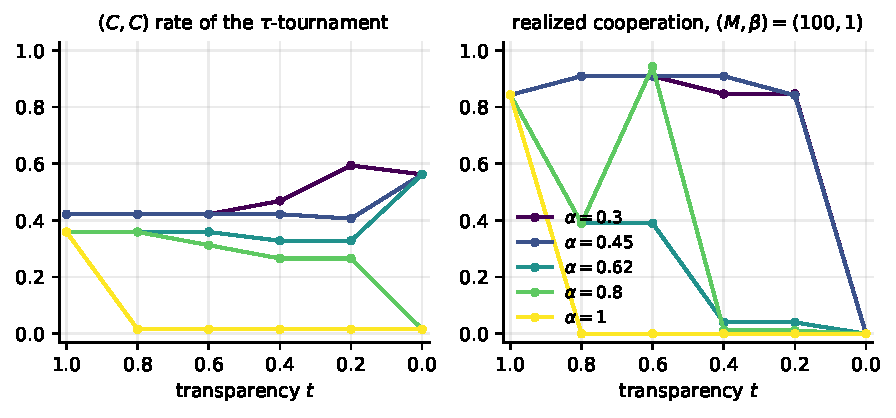
\includegraphics[width=\textwidth]{figures and tables/fig_tau_summary_body_hinge_side}
  \caption{The two analyses over transparency on the eight-bot zoo with the hinge pairs at the hinge side, behavioral family, one curve per caution $\alpha$: $(C,C)$ rate of the $\tau$-tournament (left) and realized cooperation of the evolved population at $(M,\beta)=(100,1)$ (right). Compare \cref{fig:tau-summary-body}.}
  \label{fig:tau-summary-body-hinge-side}
\end{figure}
